\documentclass[border=3pt]{standalone}
% Preâmbulo compartilhado pelos diagramas TikZ da aula 5 de IHC (Processos de Design)
\usepackage[T1]{fontenc}
\usepackage[utf8]{inputenc}
\usepackage{lmodern}
\usepackage{amsmath}
\usepackage{xcolor}
\usepackage{tikz}
\usetikzlibrary{arrows.meta,angles,quotes,decorations.pathmorphing,calc,
                positioning,shapes.geometric,shapes.misc,backgrounds,fit,
                math}

% Paleta (mesma dos SVGs originais)
% Paleta da disciplina de IHC: acento roxo (#755099), da capa do livro.
% (o nome "dblue" é mantido para não alterar todos os diagramas)
\definecolor{dblue}{HTML}{755099}
\definecolor{dorange}{HTML}{B3541E}
\definecolor{dgreen}{HTML}{4A7C59}
\definecolor{dred}{HTML}{9C4B4B}
\definecolor{dcream}{HTML}{F4F1EA}
\definecolor{dshade}{HTML}{DDD7C9}

% Função gaussiana (não normalizada por padrão de escala visual)
\pgfmathdeclarefunction{gauss}{3}{%
  \pgfmathparse{1/(#3*sqrt(2*pi))*exp(-((#1-#2)^2)/(2*#3^2))}%
}

% Estilos comuns (prefixo d... para não colidir com chaves internas do pgf)
\tikzset{
  >={Stealth[length=2mm]},
  dguide/.style={gray!55, dashed, line width=0.4pt},
  daxis/.style={gray!60, line width=0.7pt, ->},
  dbody/.style={fill=black!3, draw=black!80, line width=1pt},
  dacc/.style={draw=dblue, line width=1pt},
  dlbl/.style={black!55, font=\small},
  dsub/.style={black!45, font=\footnotesize},
  dstate/.style={circle, draw=black!80, fill=dcream, line width=1pt,
                 minimum size=17mm, font=\large, inner sep=1pt},
  dobs/.style={circle, draw=black!80, fill=dshade, line width=1pt,
               minimum size=14mm, font=\large, inner sep=1pt},
  dbox/.style={rounded corners=2pt, draw=black!80, fill=dcream, line width=1pt,
               align=center, inner sep=6pt},
  dop/.style={circle, draw=black!80, fill=white, line width=1pt,
              minimum size=6mm, inner sep=0pt, font=\small},
  dtrans/.style={->, dblue, line width=1pt},
  dmeas/.style={->, dorange, line width=1pt},
  dcurve/.style={line width=1pt, dblue},
  dcurveb/.style={line width=1.4pt, dorange},
}

\begin{document}
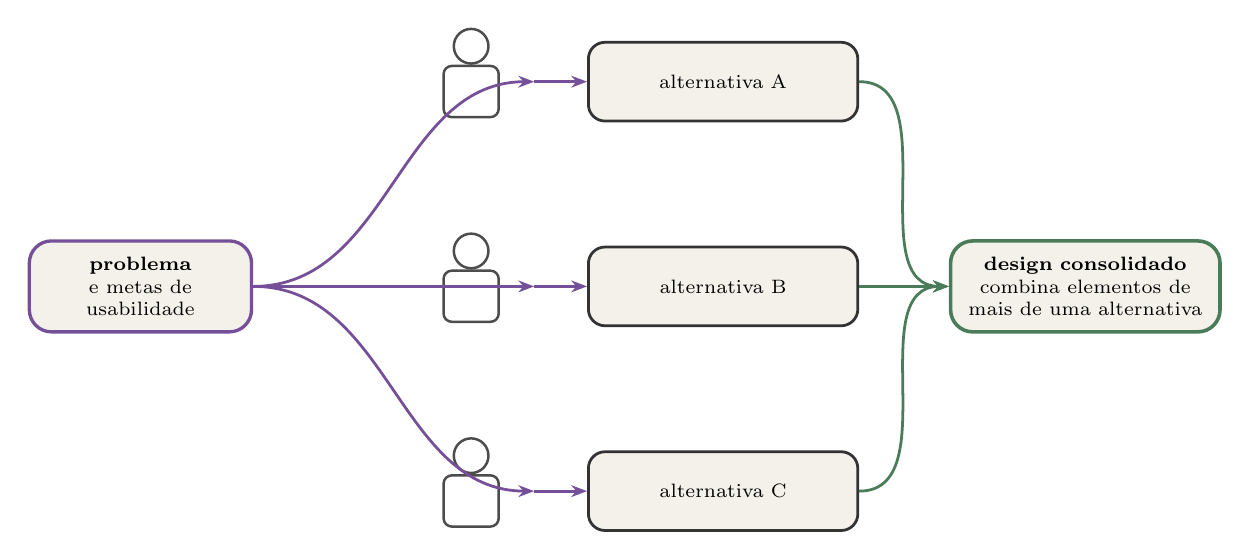
\begin{tikzpicture}[x=1cm,y=1cm,
   alt/.style={dbox, rounded corners=6pt, text width=3.0cm, minimum height=1.0cm, font=\scriptsize}]

  \node[dbox, rounded corners=8pt, text width=2.4cm, font=\scriptsize, draw=dblue, line width=1.2pt] (p) at (0,0) {\textbf{problema}\\ e metas de usabilidade};

  \foreach \y/\n in {2.6/A,0/B,-2.6/C} {
    \begin{scope}[shift={(4.2,\y)}]
      \draw[black!70, line width=0.9pt, fill=white] (0,0.45) circle (0.22);
      \draw[black!70, line width=0.9pt, fill=white, rounded corners=3pt] (-0.35,-0.45) rectangle (0.35,0.2);
    \end{scope}
    \node[alt] (a\n) at (7.4,\y) {alternativa \n};
    \draw[->, dblue, line width=1pt] (p.east) to[out=0,in=180] (5.0,\y);
    \draw[->, dblue, line width=1pt] (5.0,\y) -- (a\n.west);
  }

  \node[dbox, rounded corners=8pt, text width=3.0cm, font=\scriptsize, draw=dgreen, line width=1.3pt] (c) at (12.0,0) {\textbf{design consolidado}\\ combina elementos de mais de uma alternativa};
  \foreach \n in {A,B,C} { \draw[->, dgreen, line width=1pt] (a\n.east) to[out=0,in=180] (c.west); }


\end{tikzpicture}
\end{document}
